%%%%%%%%%%%%%%%%%%%%%%%%%%%%%%%%%%%%%%%%%%%%%%%%%%%%%%%%%%%%%%%%
%%%%%%%%%%%%%%%%%%%%%%%%%%%%%%%%%%%%%%%%%%%%%%%%%%%%%%%%%%%%%%%%
%%%%
%%%% This text file is part of the source of 
%%%% `The Art of HPC, vol 1: The Science of Computing'
%%%% by Victor Eijkhout, copyright 2012-2022
%%%%
%%%% This book is distributed under a Creative Commons Attribution 3.0
%%%% Unported (CC BY 3.0) license and made possible by funding from
%%%% The Saylor Foundation \url{http://www.saylor.org}.
%%%%
%%%% hpc_linear.tex : linear algebra
%%%%
%%%%%%%%%%%%%%%%%%%%%%%%%%%%%%%%%%%%%%%%%%%%%%%%%%%%%%%%%%%%%%%%
%%%%%%%%%%%%%%%%%%%%%%%%%%%%%%%%%%%%%%%%%%%%%%%%%%%%%%%%%%%%%%%%

\documentclass[11pt]{beamer}

\beamertemplatenavigationsymbolsempty
\usepackage{beamerthemeTACC}
\parskip=.5\baselineskip plus .5\baselineskip
\input semester

\usepackage{pslatex}
\usepackage{amsmath,comment,multirow,multicol} %% ,arydshln

\newdimen\unitindent \unitindent=20pt

\input slidemacs

\input scimacs

\excludecomment{diagonalstorage}

\begin{document}
\parskip=10pt plus 5pt minus 3pt

\title{Numerical Linear Algebra}
\author{\hpcteachers}
\date{\hpcsemester}

\begin{frame}
  \titlepage
\end{frame}

\begin{frame}{Justification}
  Many algorithms are based in linear algebra, 
  including some non-obvious ones such as graph algorithms.
  This session will mostly discuss aspects of 
  solving linear systems, focusing on those
  that have computational ramifications.
\end{frame}

\input LinearAlgebra-slides

\sectionframe{Short detour: Partial Differential Equations}

\begin{frame}{Second order PDEs; 1D case}
  \onslide<1->{
    \[ 
    \begin{cases}
      -u''(x)=f(x)&x\in[a,b]\\
      u(a)=u_a,\,u(b)=u_b
    \end{cases}
    \]
  }
  \onslide<2->{
    \footnotesize
    Using Taylor series:
    \[ u(x+h)+u(x-h)=2u(x)+u''(x)h^2+u^{(4)}(x)\frac{h^4}{12}+\cdots \]
    so
    \[ u''(x)=\frac{u(x+h)-2u(x)+u(x-h)}{h^2} +O(h^2) \]
    Numerical scheme:
    \[ -\frac{u(x+h)-2u(x)+u(x-h)}{h^2}=f(x,u(x),u'(x)) \]
  }
\end{frame}

\frame{\frametitle{This leads to linear algebra}
  \[ -u_{xx}=f\rightarrow
  \frac{2u(x)-u(x+h)-u(x-h)}{h^2}=f(x,u(x),u'(x)) 
  \]
  Equally spaced points on $[0,1]$: $x_k=kh$ where $h=1/(n+1)$, then
  \[ -u_{k+1}+2u_k-u_{k-1} = -h^2\,f(x_k,u_k,u'_k)
  \quad\hbox{for $k=1,\ldots,n$} \]
  Written as matrix equation:
  \[
  \left(
    \begin{matrix}
      2&-1&&\emptyset\\
      -1&2&-1\\
      \emptyset&\ddots&\ddots&\ddots
    \end{matrix}\right)
  \left(
    \begin{matrix}
      u_1\\ u_2\\ \vdots
    \end{matrix}\right)
  =
  \left(
    \begin{matrix}
      f_1+u_0\\ f_2\\ \vdots
    \end{matrix}\right)
  \]
}

\begin{frame}{Second order PDEs; 2D case}
  \[
  \begin{cases}
    -u_{xx}(\bar x)-u_{yy}(\bar x)=f(\bar x)&x\in\Omega=[0,1]^2\\
    u(\bar x)=u_0&\bar x\in\delta\Omega
  \end{cases}
  \]
  Now using central differences in both $x$ and $y$ directions.
\end{frame}

\begin{frame}{The stencil view of things}
  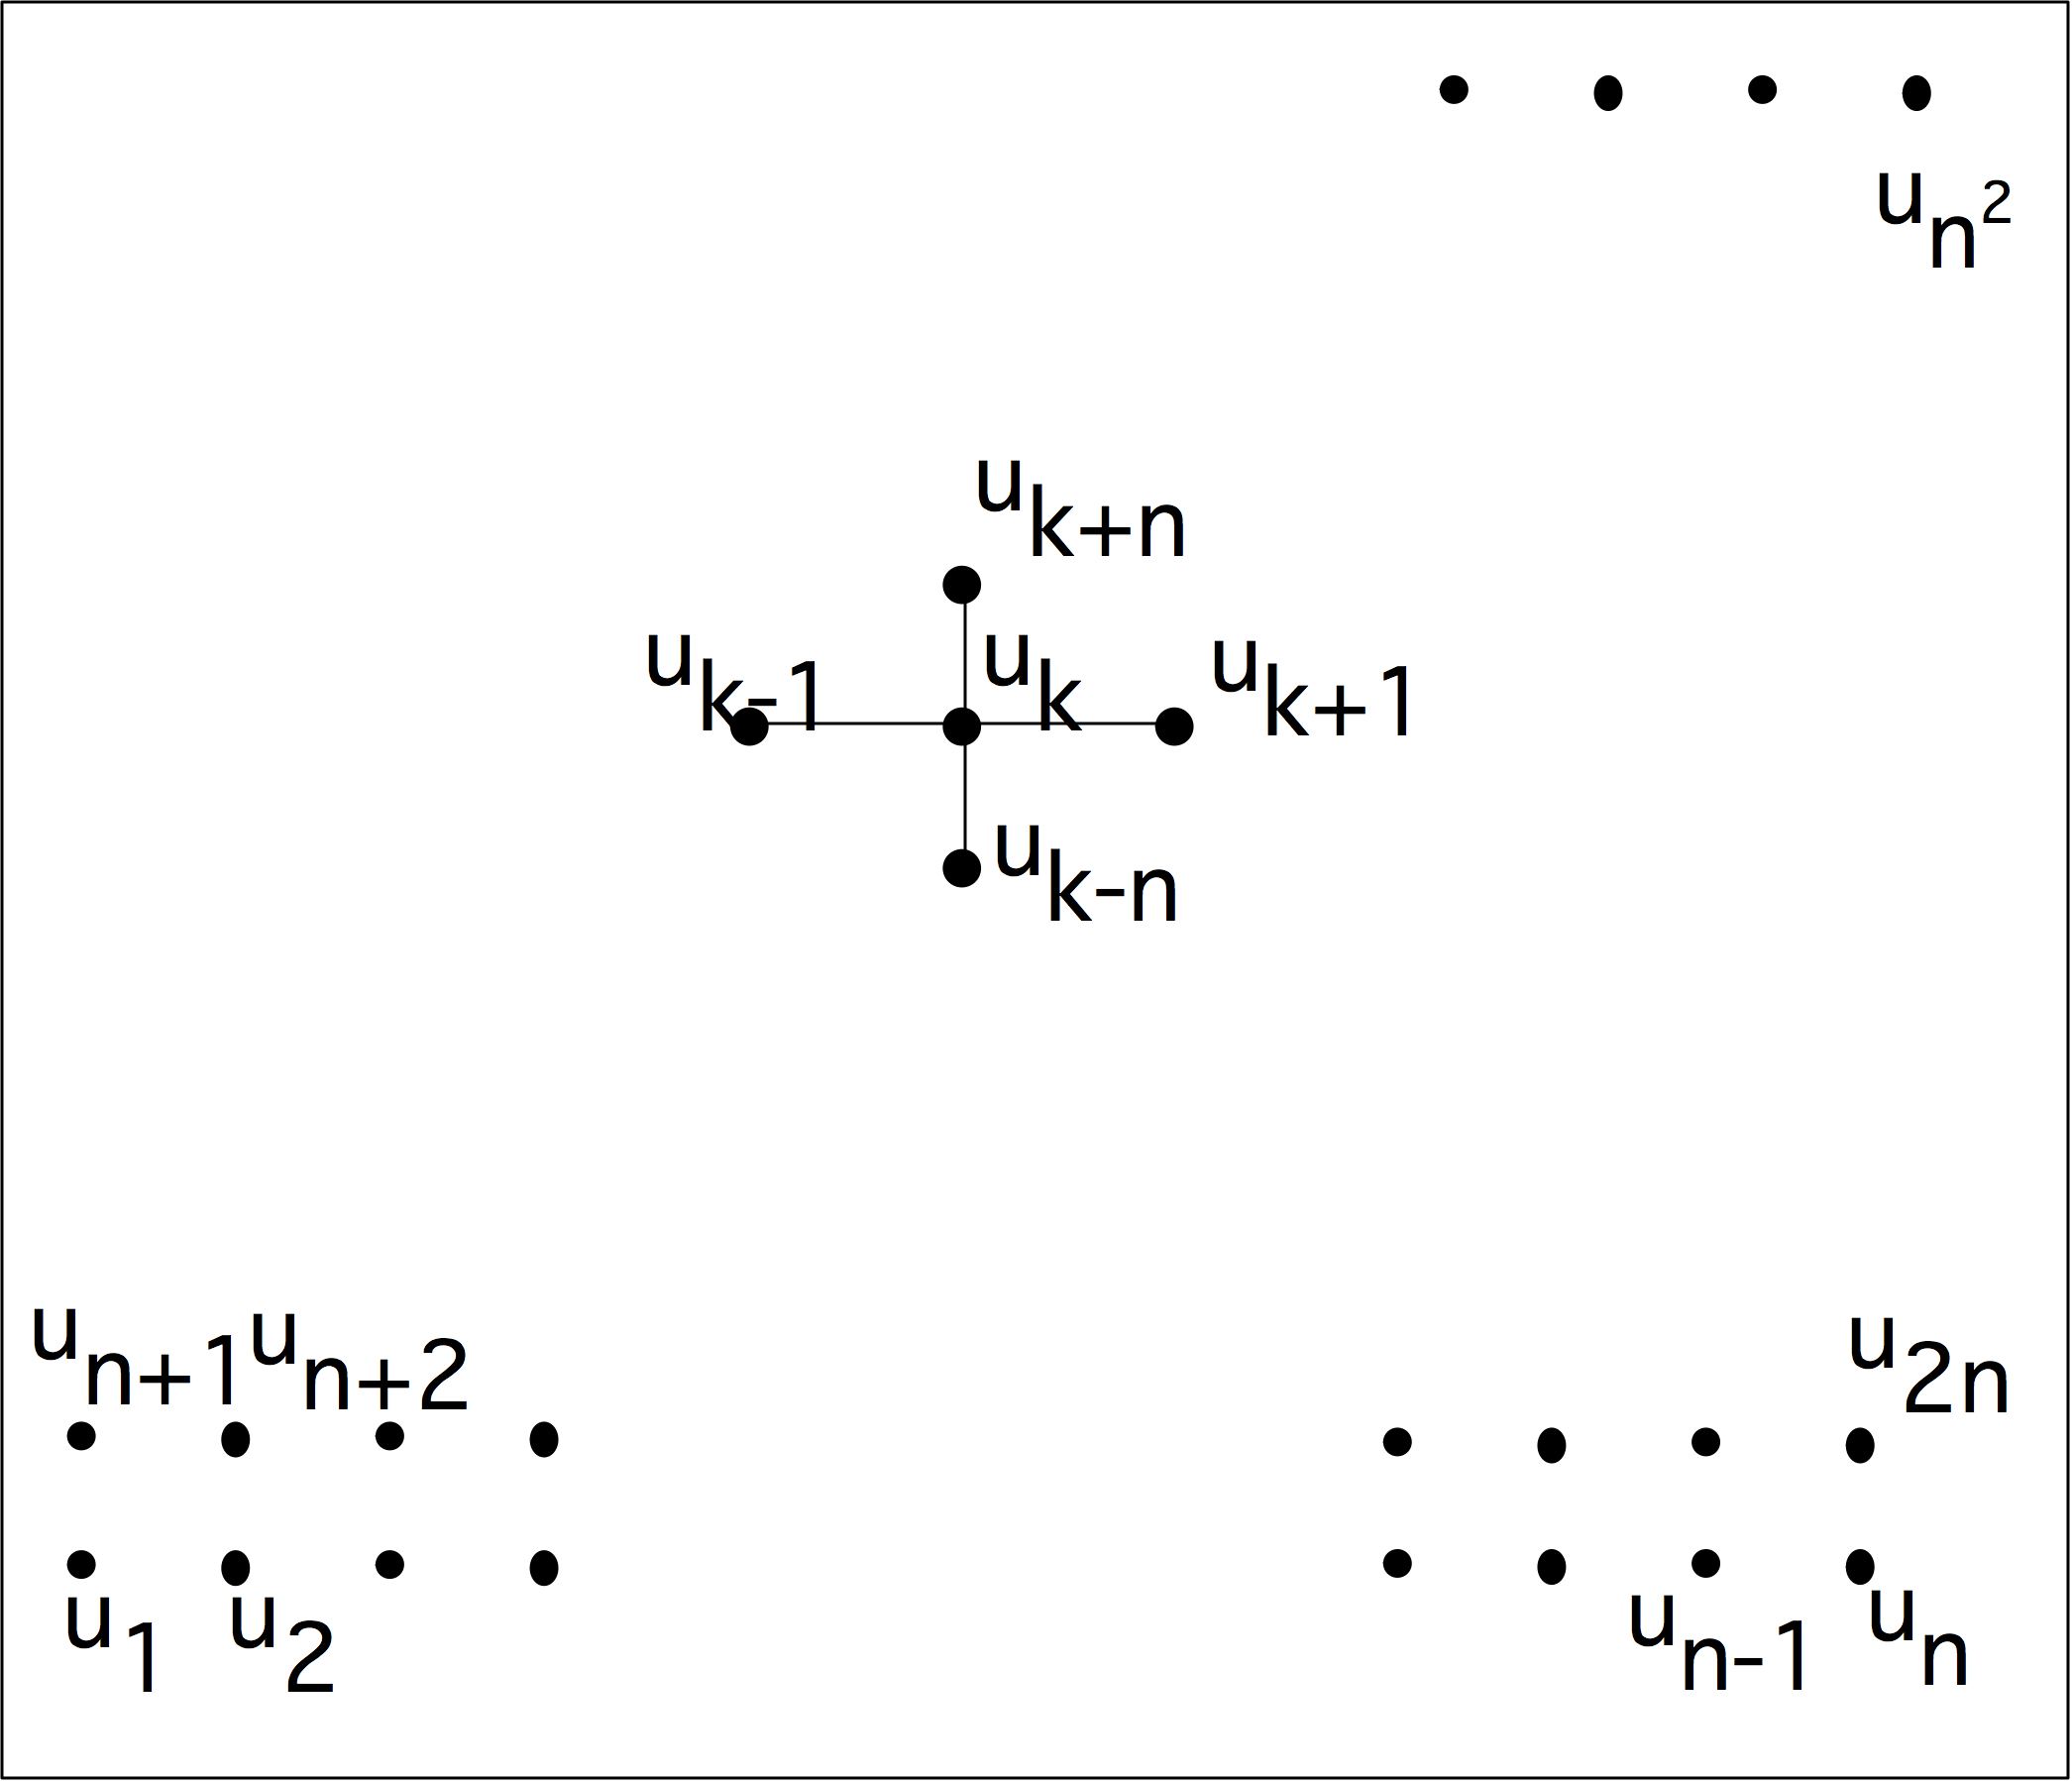
\includegraphics[scale=.1]{laplacedomain}
\end{frame}

\frame{\frametitle{Sparse matrix from 2D equation}
  \small
  \[
  \left(\begin{array}{ccccc|ccccc|cc}
    4&-1&&&\emptyset&-1&&&&\emptyset&\\ 
    -1&4&1&&&&-1&&&&\\ 
    &\ddots&\ddots&\ddots&&&&\ddots&&\\ 
    &&\ddots&\ddots&-1&&&&\ddots&\\ 
    \emptyset&&&-1&4&\emptyset&&&&-1&\\ \hline
    -1&&&&\emptyset&4&-1&&&&-1\\
    &-1      &      &&&-1      &4       &-1      &&&&-1\\
    &\uparrow&\ddots&&&\uparrow&\uparrow&\uparrow&&  &&\uparrow\\
    &k-n     &      &&&k-1     &k       &k+1     &&-1&&k+n\\
    &&&&-1&&&&-1&4&&\\ \hline
    &        &      &&&\ddots  &        &        &&  &\ddots\\
  \end{array}\right)
  \]
  The stencil view is often more insightful.
}

\frame{\frametitle{Matrix properties}

  \begin{itemize}
  \item Very sparse, banded
  \item Factorization takes less than $n^2$ space, $n^3$~work
  \item Symmetric (only because 2nd order problem)
  \item Sign pattern: positive diagonal, nonpositive off-diagonal\\
    (true for many second order methods)
  \item Positive definite (just like the continuous problem)
  \item Constant diagonals: only because of the constant coefficient
    differential equation
  \item Factorization: lower complexity than dense, recursion length less than~$N$.
  \end{itemize}
}

\sectionframe{Sparse matrices}

\input SparseMatrices-slides

\end{document}
